{\let\cleardoublepage\relax \chapter{Przyswajanie wiedzy}}

\todo[inline]{Jeśli opisuje coś na podstawie strony internetowej pana Doktora to czy to jest plagiat?}

Hermann Ebbinghaus\cite{HumanMemory} (1850-1909) był Niemieckim psychologiem, który jako jeden z pierwszych zajmował się tematyką eksperymentalnej psychologii związanej z przyswajaniem wiedzy. 
Jednym z jego pierwszych eksperymentów było stworzenie testu, podczas którego uczył się zestawu 20 sylab, które były bezsensowne ze względu na fakt, iż w jego języku nie występowały żadne słowa, które ich używały.
Eksperyment ten pozwolił mu skonstruować pierwszą na świecie krzywą zapominania. Miała ona charakter eksponencjalny.  Możemy z niej wywnioskować, iż podczas początkowego okresu zapominania tracimy najwięcej zapamiętanych informacji.

\begin{figure}[h]
	\centering
	\includegraphics[width=\textwidth]{images/curve.png}
	 \caption{Eksponencjalna krzywa zapominania.}
\end{figure}

Trzeba także zwrócić uwagę na fakt, iż w rzeczywistości\cite{ForgettingCurve} nasz mózg nie jest w stanie przyswoić danych informacji w 100\% po zakończeniu nauki. 

\section{Interwały potwórzeń}

W celu jak najlepszego zapamiętania wyuczonych informacji należy, poza odpowiednim programem nauczania, zwrócić uwagę na fakt w jakich interwałach czasowych powtarzamy przerabiany materiał\cite{ForgettingCurve}.
Interwał musi być wystarczająco krótki aby zapobiec zapominaniu i wystarczająco długi, aby zbyt często nie przyswajać powtarzanego materiału.



\todo[inline]{Można tu jeszcze coś napisać}



{\let\cleardoublepage\relax \chapter{.NET}}
\label{cha:wstep}

%https://docs.microsoft.com/en-us/dotnet/standard/tour
.NET jest platformą programistyczną umożliwiającą pisanie nowoczesnych aplikacji w językach wysokiego poziomu, do których zalicza się m.in C\# , VB oraz F\#. Platforma ta wyróżnia się tym iż:
\begin{itemize}
	\item Pozwala na użycie wielu języków programowania podczas pisania naszych programów
	\item Ma zaimplementowane mechanizmy do obsługi operacji asynchronicznych i współbieżnych
	\item Można ją stosować na różnych platformach, które posiadają środowisko wykonywalne .NET
\end{itemize}
Wszystkie języki używane w platformie .NET kompilowane są do Wspólnego Języka Pośredniego (po ang. \textit{Common Intermediate Language}), który następnie jest tłumaczony na kod bajtowy i wykonywany za pomocą środowiska wykonywalnego danej implementacji .NET.

\begin{lstlisting}[frame=single, numbers=none,captionpos=b, 
caption={Przykładowy kod aplikacji "Hello World" w języku CIL}]
.assembly HelloWorld
.class auto ansi HelloWorldApp
{
     .method public hidebysig static void Main() cil managed
     {
          .entrypoint
          .maxstack 1
          ldstr "Hello world."
          call void [mscorlib]System.Console::WriteLine(string)
          ret
     }
}
\end{lstlisting}

%https://docs.microsoft.com/en-us/dotnet/standard/tour
% CLI ECMA http://www.ecma-international.org/publications/files/ECMA-ST/ECMA-335.pdf

\section{Implementacje .NET}

Każda aplikacja .NET jest uruchamiana na jednej z implementacji .NET. \\
Od roku 2016 wprowadzono .NET Standard - wspólny zestaw API, które każda z implementacji musi posiadać. Pozwala to na pisanie i używanie bibliotek programistycznych w różnych środowiskach .NET.

Istnieją aktualnie 4 główne implementacje .NET:

%https://docs.microsoft.com/en-us/dotnet/standard/components
\subsection{.NET Core}
Został napisany z myślą o tworzeniu aplikacji cross-platformowych, które mogą zostać uruchomione na serwerach, jak i środowiskach chmurowych. Potrafi działać na platformie Windows, macOS oraz Linux. Jest to pierwsza implementacja .NET, która została zaprojektowana przez Microsoft z myślą o wieloplatformowości.

%https://docs.microsoft.com/en-us/dotnet/framework/get-started/overview
\subsection{.NET Framework}
Jest to pierwsza, oryginalna implementacja .NET, która istnieje od roku 2002. Składa się ze środowiska uruchomieniowego Common Language Runtime (CLR) oraz biblioteki standardowej zwanej jako Framework Class Library (FCL). CLR zapewnia aplikacjom wirtualną maszynę, na której wykonywany kod bajtowy skompilowany z języka CIL. Ta implementacja jest używana w tej pracy inżynierskiej.

%http://www.mono-project.com/docs/about-mono/
\subsection{Mono}
Darmowy projekt open-source prowadzony przez firmę Xamarin. Powodem stworzenia tego produktu była możliwość uruchamiania aplikacji napisanych w językach .NET na wielu platformach, jak i dostarczenie użytkownikom Linuxa narzędzi pozwalających na aplikacji w rodzinie języków .NET.
%https://docs.microsoft.com/en-us/windows/uwp/get-started/whats-a-uwp
\subsection{Universal Windows Platform (\textit{UWP})}
Implementacja, która umożliwia tworzenie aplikacji dla wszystkich platform używających Windows 10, Xboxa, niektórych urządzeń stworzonych przez Microsoft i dostosowanych urządzeń IoT.

{\let\cleardoublepage\relax \chapter{ASP.NET MVC}}
\label{cha:wstep}
%https://msdn.microsoft.com/en-us/library/dd381412(v=vs.108).aspx

ASP.NET MVC jest frameworkiem do budowania aplikacji internetowych w oparciu o wzorzec architektoniczny Model-View-Controller (MVC). Wykorzystuje implementacje .NET Framework do uruchamiania skompilowanego kodu źródłowego.


\section{Model-Widok-Kontroler}

Większość dzisiejszych systemów komputerowych działa na zasadzie wyświetlania danych, które aktualnie znajdują się w bazie danych i ewentualna ich modyfikacja. Z tego też powodu narodził się wzorzec Model-Widok-Kontroler(ang. Model-View-Controller), który rozdziela logikę aplikacji na 3 główne segmenty:
\begin{enumerate}
	\item Model - Służy do przechowywania danych, pobierania danych i ich ewentualnej zmiany na podstawie zapytań z kontrolera.
	\item Kontroler - przetwarza zapytania użytkownika, które przekazuje do modelu, który jest następnie wyświetlany jako widok.
	\item Widok - Służy do wyświetlania informacji 
\end{enumerate}

% Framework do budowania stron internetowych w oparciu o technologie .NET
\begin{figure}[h]
	\centering
	\includegraphics[height=50.5mm]{images/mvc.png}
	 \caption{Podać źródło}
\end{figure}

Cała moja aplikacja została skonstruowana zgodnie z tym wzorcem projektowym. ASP.NET MVC, jak już sama nazwa wskazuje, bardzo mocno opiera się na nim. Dostarczana jest klasa bazowa \textbf{Controller}, która dostarcza wszystkie podstawowe metody do wyświetlania odpowiednich treści danych i zarządzania zapytaniami.
Całe to rozwiązanie niesie za sobą korzyści związane z warstwą wyświetlania prezentowanych danych. Jest to warstwa aplikacji, w której bardzo często dochodzi do zmian. Dzięki podejściu MVC i odseparowaniu danych od widoku jesteśmy w stanie tworzyć jak i zmieniać widoki, bez wpływu na kod biznesowy aplikacji.

\section{Wzorzec Repozytorium\cite{RepositoryUnitOfWorkPattern}}

Wewnątrz naszej aplikacji będziemy używać bazy danych Microsoft SQL. Bardzo często jest tworzony kod, którego celem jest zwrócenie bardzo podobnych danych. W celu zmniejszenia redundancji kodu jak i odseparowania zależności i odpowiedzialności wykorzystałem wzorzec Repozytorium (z ang. Repository Pattern).

Wzorzec ten wykorzystuje obiekty, zwane repozytoriami, których jedynym zadaniem jest pobieranie i modyfikowanie danych po stronie serwera SQL. Nie zawierają żadnej logiki biznesowej i są niezwiązane z resztą kodu danej aplikacji. 

\begin{figure}[h]
	\centering
	\includegraphics[width=\textwidth]{images/RepositoryPattern.png}
	 \caption{Wzorzec repozytorium. Źródło: msdn.microsoft.com}
\end{figure}

Wewnątrz mojego projektu cały wzorzec repozytorium został oparty na interfejsach \textbf{IRepository} i \textbf{IRepository<T>} (który implementuje \textbf{IRepository}). W założeniu te interfejsy mówią jedynie o tym jakie operacje można zrealizować na danym obiekcie klasy 'T'. Informacje o tym jak te informacje są realizowane jak i to, iż są one realizowane za pomocą bazy danych Microsoftu są przechowywane w klasie \textbf{RepositoryBase<T>}.
Wszystkie kolejne stworzone repozytoria dziedziczą po \textbf{RepositoryBase<T>} a ich interfejsy implementują \textbf{IRepository<T>}. Takie działanie pozwala nam na brak ścisłego powiązania naszych repozytoriów z bazą danych Microsoft SQL. Wystarczy iż zmienimy \textbf{RepositoryBase<T>} na jakąkolwiek inną klasę implementującą \textbf{IRepository<T>} i wykorzystamy ją w naszych repozytoriach. Dzięki temu małym nakładem siły moglibyśmy zastąpić Microsoft SQL danymi zapisywanymi w pamięci RAM naszego komputera wewnątrz wyspecjalizowanych kolekcji. 


\begin{figure}[h]
	\centering
	\includegraphics[width=\textwidth]{images/ReviewRepository.png}
	 \caption{Repozytorium ReviewCardRepository wraz z implementowanymi interfejsami i odziedziczonymi klasami.}
\end{figure}

\section{Jednostka Pracy\cite{RepositoryUnitOfWorkPattern}}
%https://docs.microsoft.com/en-us/aspnet/mvc/overview/older-versions/getting-started-with-ef-5-using-mvc-4/implementing-the-repository-and-unit-of-work-patterns-in-an-asp-net-mvc-application

Wzorzec Jednostki Pracy (z ang. Unit of Work) ma na celu uporządkowanie pracy z repozytoriami za pomocą umieszczenia ich wszystkich w jednej klasie. Dodatkowo wszystkie repozytoria współdzielą kontekst dostępu do bazy danych. Zapisanie danych odbywa się poprzez wywołanie metody \textbf{SaveChanges} wewnątrz Jednostki Pracy (SaveChanges jest konwencją wewnątrz mojego projektu).

\begin{figure}[h]
	\centering
	\includegraphics{images/UnitOfWork.png}
	 \caption{Jednostka pracy wykorzystywana w projekcie.}
\end{figure}

\section{Mapowanie obiektowo-relacyjne}

Wewnątrz mojego projektu wykorzystałem narzędzie Entity Framework, które pozwala na korzystanie z mapowania obiektowo-relacyjnego. Dzięki tej technicę mogę uprzednio zdefiniowane dane tabelaryczne odzworować za pomocą klas, które zostaną stworzone na podstawie definicji tabeli i relacji między nimi. Powstałe klasy są używane wewnątrz kolekcji, implementujących interfejs \textbf{IQueryable<T>}, na których możemy wykonywać zapytania z pomocą \textbf{LINQ}a. 
\\ \\
Takowe rozwiązanie ma wiele zalet :
\begin{enumerate}
	\item Dane z danej tabeli będziemy mogli otrzymać zawsze w tym samym formacie. Unika się dzięki temu sytuacji gdzie dana tabela ma wiele odpowiadających jej klas w kodzie, które służą jedynie do dostępu do danych.
	\item W przypadku zmiany typu w tabeli typ ten możemy bardzo prosto zmienić w kodzie.
	\item Zmniejsza to zakres potrzebnych umiejętności w celu używania danych występujących w bazie danych. Dany programista nie musi znać języka SQL, aby w sposób bezproblemowy pobrać interesujące go dane, nawet gdy tworzy bardzo skomplikowane zapytania.
	\item Łatwiejsza nawigacja po zależnościach między tabelami. Na danym typie możemy na przykład wykorzystać operacje \textbf{Find All References}, która wskaże nam użycia danego typu w naszym kodzie. W przypadku kodu SQL nie mielibyśmy takiej możliwości.
\end{enumerate}

\section{Wstrzykiwanie zależności}

Wstrzykiwanie zależności (%ang. Dependency Injection) jest wzorcem projektowym, który jest łatwy do wykorzystywania wewnątrz aplikacji pisanych w ASP.NET MVC. Jego działanie polega na tym, iż obiekty naszej aplikacji nie muszą tworzyć zależnych od siebie obiektów, lecz są tworzone przez obiekt nadrzędny dla użytku tych klas. 

Informacja o tym, iż dana klasa ma zamiar używać instancji innej klasy może być zawarta poprzez odpowiednie wywołanie danej funkcji, bądź poprzez użycie listy interfejsów w konstruktorze, która zostanie wypełniona odpowiednimi instancjami.

W przypadku mojej aplikacji użyłem do tego biblioteki Ninject\cite{NinjectGithub}. Jest to bardzo popularna biblioteka realizująca wzorzec wstrzykiwania zależności. Dzięki niej możemy zdefiniować listę potrzebnych interfejsów/klas jako parametry konstruktora naszego kontrolera, a te utworzą się automatycznie podczas żądania użytkownika. Jeśli tworzone klasy także będą wymagały do swojego istnienia pewnych interfejsów bądź klas i zostanie to uściślone w ich konstruktorze to także dla nich zostaną dostarczone odpowiednie instancje.
\\ \\
Jednakże sam interfejs nie daje żadnej informacji o tym, jaką klasę należy zinstancjować, ponieważ może być wykorzystywany przez wiele klas pochodnych. W tym celu należy poinformować Ninject o tym, jakie klasy mają zostać zinstancjonowane poprzez zbindowanie interfejsów do odpowiednich klas. To działanie jest przedstawione na poniższym listingu:

\begin{lstlisting}[frame=single, numbers=none,captionpos=b, 
caption={Przykładowy kod bindowania dla biblioteki Ninject}]
public static void RegisterServices(IKernel kernel)
{
kernel.Bind<FlashcardsEntities>().ToSelf().InRequestScope();
kernel.Bind<IFlashcardRepository>().To<FlashcardRepository>().InRequestScope();
}
\end{lstlisting}

Jak widzimy proces pojedynczego bindowania możemy podzielić na 2 części:

\begin{enumerate}
	\item Informacja o tym co powinno zostać stworzone przez Ninject gdy jest proszone o daną klasę
	\item Informacja o zasięgu współużywania danej instancji.
\end{enumerate}

\begin{figure}[h]
	\centering
	\includegraphics[width=\textwidth]{images/ninject.png}
	 \caption{Proces bindowania z wyszczególnionymi częściami składowymi}
\end{figure}

Wewnątrz pierwszej części określamy jakim typem ma zostać zastąpiony dany typ w procesie wstrzykiwania. Na przykładzie widzimy, że typ może "zastąpić" sam siebie bądź może zostać użyty inny typ, który będzie jego instancją. Należy pamiętać, iż ten drugi typ musi implementować, dziedziczyć bądź być tym samym typem co pierwszy.
\\
%Fajnie tutaj byłoby to dać w jakąś ramkę czy coś
Ninject dodatkowo potrafi zbindować dany typ do \textbf{metody} lub klasy implementującej interfejs \textbf{Provider<T>}. Taka metoda, badź klasa musi zwrócić w wyniku swojego działania pełnoprawny obiekt danego typu.


%https://github.com/ninject/ninject/wiki/Object-Scopes
Ninject w swoim domyślnym zachowaniu za każdym razem jak poprosimy go obiekt danej klasy to tworzony jest następny obiekt danej klasy. Jednakże często dochodzi do sytuacji, że w danym segmencie kodu chcielibyśmy aby obiekt danej klasy był współdzielony między wszystkimi instacjami wytworzonymi przez Ninject. Wtedy za każdym razem jak poprosimy obiekt klasy A to zawsze w ramach danego zasięgu dostaniemy ten sam obiekt i nie zostanie on utworzony ponownie.
Jest to szczególnie przydatne w środowisku serwerowym, gdy chcemy aby dla każdego zapytania klienta wszystkie repozytoria i serwisy były zawsze takie same. Nie tylko nie ponosimy kosztów utworzenia danej instancji, lecz także współdzielone repozytoria mogą szybciej zwracać informacje odnośnie danych po stronie serwera SQL gdy zobaczą iż mają te dane w swoim cache'u.

\newpage
{\let\cleardoublepage\relax \chapter{Testy}}

Bardzo ciężko jest napisać w dzisiejszym świecie aplikację nie zaopatrując się w zestaw testów bądź innych mechanizmów sprawdzających poprawność wykonania kodu. Z tego też powodu napisałem duży zestaw testów jednostkowych, które sprawdzają, czy pojedyncze funkcjonalności danych serwisów są funkcjonalne. 

\section{Testy Jednostkowe}

Odwołania do innych serwisów/obiektów w większości zastąpiłem za pomocą atrap obiektów (z ang. mock object), które zastępują wywołania danych funkcjonalności poprzez zwrócenie domyślnych wartości. Możemy także zastąpić daną funkcjonalność atrapy jakąś mało skomplikowaną logiką w celach testowych. Taka atrapa nie dość, iż potrafi odłączyć nasz obiekt od reszty systemu, przez co jesteśmy w stanie testować go jednostkowo to dodatkowo zawiera bardzo dużo funkcjonalności pomagających zweryfikować czy dany test przebiegł poprawnie. W celu tworzenia atrap wykorzystałem framework Moq\cite{MoqGithub}.



Większość, jeśli nie wszystkie testy zostały ułożone zgodnie ze wzorcem AAA\cite{UnitTestingMicrosoft} - Aranżacja (z ang. Arrange) Akcja (z ang. Act) Asercja (z ang. assert). Takie ułożenie testów sprawia, iż testy są konsystentne i czytelne. Potrzebujemy bardzo małej ilości czasu, aby zaznajomić się z danym testem.


\begin{lstlisting}[frame=single, numbers=none,captionpos=b, 
caption={Przykładowy test jednostkowy wykorzystujący metodę AAA}]
public void StopLastTraining_assert_tests()
{
	//Aranżacja - stworzenie wewnętrznej atrapy obiektu dla atrapy serwisu
	mockTraining();
	//Akcja
	trainingReviewService.StopLastTraining();
	//Asercja - sprawdzenie poprawności wykonania
	trainingRepository.Verify(x => x.Remove(It.IsAny<long>()), Times.Once);
	unit.Verify(x => x.SaveChanges(), Times.Once); //wykorzystanie funkcjonalności frameworku Moq w celu sprawdzenia czy dana metoda została wywołana.
	Assert.AreEqual(null, sessionService.Object.UserInfo.TrainingInfo);
}
\end{lstlisting}

\section{Testy Integracyjne}
%Czy to jest potrzebne???
\todo[inline]{Czy ten fragment jest potrzebny? Omawiam tutaj co prawda część aplikacji, lecz niestety nie jest on de facto wykorzystywany przeze mnie}
Dla potrzeb porzuconej części aplikacji został także napisany mały zestaw testów integracyjnych testujących serwis do obsługi zapisu i odczytu plików XML, jak i test tworzenia tymczasowych plików w systemie Windows. 
Testy te miały za zadanie testować współdziałanie powyższych funkcjonalności z zewnętrznymi komponentami nieobsługiwanymi przez moją aplikację. Z tego też powodu nie został tutaj wykorzystany framework do tworzenia atrap. Wszystkie testy, pomimo tego, iż poprawne to aktualnie nie dowodzą poprawności żadnego elementu aktualnie używanej aplikacji, ponieważ były wykorzystywane przez porzuconą część aplikacji.



\newpage
{\let\cleardoublepage\relax \chapter{Kaskadowe Arkusze Styli}}

W moim projekcie wykorzystuję tzw. Kaskadowe Arkusze Styli \cite{CSSDoc}. Ich przeznaczeniem jest stylizować wygląd wyświetlanej strony HTML dla użytkownika. Pewne fragmenty strony są odnajdywane dzięki selektorom i są formatowane według reguł zdefiniowanych dla danego selektora. To pozwala nam na ponowne użycie tych samych styli w obrębie naszych aplikacji, dzięki zdefiniowaniu bardziej uogólnionych selektorów.

\section{Syntaktycznie Zarąbiste Arkusze Styli}

W dzisiejszym świecie nikt obeznany z technologią tworzenia stron internetowych nie używa już czystego języka CSS do tworzenia styli. Przy tworzeniu styli dla danej strony stykamy się z bardzo dużą redundancją kodu, która jest związana z tym iż pewne fragmenty strony wyglądają zawsze tak samo (np. motyw kolorystyczny dla większości elementów jest ten sam). Brak zmiennych w języku CSS powoduje, iż zmiana kolorystyki strony jest żmudnym i ciężkim zadaniem.
Z tego tez powodu wykorzystuję język SASS - Syntactically Awesome Style Sheets (Syntaktycznie Zarąbiste Arkusze Styli)\cite{Sass}. Jest on kompatybilny ze wszystkimi wersjami CSS. Co powoduje, iż każdy kod napisany w CSS jest zgodny z językiem SASS. 
Sass oferuje nam bardzo dużo funkcjonalności, między innymi:
\begin{enumerate}
	\item Zmienne - dane wartości możemy zapisywać jako zmienne i używać ich wielokrotnie w obrębie naszych plików.
	\item Zagnieżdżanie - możemy zagnieżdżac selektory wewnątrz siebie. Odwzorowywuje to naturę plików HTML, przez co kod jest bardziej czytelny.
	\item Możliwość załączania innych plików. Pozwala to na logiczne podzielenie arkuszy styli.
	\item Mixin - Pozwala na tworzenie grup deklaracji, które można ponownie wykorzystać w danym stylu.
	\item Dziedziczenie - potrafimy za pomocą słówka kluczowego \textbf{@extend} odziedziczyć właściwości danego selektora.
	\item Operatory - Możemy wykorzystywać znaki \textbf{+}, \textbf{-}, \textbf{*}, \textbf{/}, \textbf{\%} do operacji na liczbach.
\end{enumerate}


\begin{lstlisting}[frame=single, numbers=none,captionpos=b, 
caption={Przykładowy kod SCSS wykorzystujący mixin}]
@mixin border-radius($radius) {
  -webkit-border-radius: $radius;
     -moz-border-radius: $radius;
      -ms-border-radius: $radius;
          border-radius: $radius;
}

.box { @include border-radius(10px); }
\end{lstlisting}

\newpage
{\let\cleardoublepage\relax \chapter{Scala\cite{ScalaWiki}}}

Scala jest językiem programowania ogólnego zastosowania, który został wprowadzony na rynek przez Laboratorium "École Polytechnique Fédérale de Lausanne". Jest to język, który jest kompilowany bezpośrednio do kodu bajtowego Javy, co powoduje, iż programy w nim napisane z łatwością uruchamiają się w środowisku wykonywalnym maszyny wirtualnej Javy. 
Scala jest językiem wielo-paradygmatowym\cite{ScalaTour}. Korzysta z dobrodziejstw programowania funkcjonalnego i obiektowego.

\begin{lstlisting}[frame=single, numbers=none,captionpos=b, 
caption={Hello world napisany w języku Scala.}]
object HelloWorld {
  def main(args: Array[String]): Unit = {
    println("Hello, world!")
  }
}
\end{lstlisting}

\section{Javascript}

Mankamentem tworzenia aplikacji webowych jest używanie Javascriptu. Coraz większa rzesza programistów odchodzi od jego używania na rzecz innych języków, które są kompilowalne do niego, takich jak np. Typescript, Coffescript, bądź jak w moim przypadku Scala.JS. Taka zmiana pozwala nam popełniać o wiele mniej błędów pisząc kod. Pomimo tego, iż wynikowym kod nadal będzie w tym samym języku.
Wszystko jest spowodowane przez to, iż Javascript posiada:
\begin{enumerate}
	\item Niejawne rzutowania, które objawiają się przy użyciu operatora ==. Są przyczyną wielu trudnych do odkrycia błędów
	\item Automatyczne wstawianie średników, co może spowodować, iż program działa inaczej niż zamierzał to programista. Czasami potrafi to uratować program napisany przez programistę, lecz często prowadzi do dziwnych i niezrozumiałych błędów, takich jak w przypadku poniższego listingu: \ref{lst:javascriptSUCKS}
	\item Niezrozumiałe zachowana różnych funkcji. Metoda sortująca będzie domyślnie sortowała tablice liczb w porządku alfabetycznym nie zwracając uwagi na fakt, iż w tablicy nie występuje ani jeden ciąg znakowy.
	\item Zmienne, którym możemy w każdej chwili zmienić typ przechowywanej wartości. Z tego też powodu bardzo często powstają prozaiczne błędy, gdzie programista oczekując liczby w danym miejscu otrzymał ciąg znakowy co skutkuje błędem w dalszym kodzie programu.
\end{enumerate}

\begin{lstlisting}[label={lst:javascriptSUCKS},
frame=single, numbers=none,captionpos=b, 
caption={Przykład niepoprawnego kodu Javascript wynikłego z automatycznego wstawienia średnika}]
function foo() {
    return // Tutaj zostanie wstawiony średnik.
        {
            bar : "test"
        };
}
\end{lstlisting}



\begin{figure}[h]
	\centering
	\includegraphics{images/javagod.png}
	 \caption{Przykład dziwnego zachowania języka. Źródło: devrant.com}
\end{figure}

\todo[inline]{Chyba jak cytuję obrazek muszę dać pełne źródło jako [x] + na samym dole odnośnik}

\section{Scala w wersji JS}

Z powodu powyższych problemów zdecydowałem się na użycie scali, która z pomocą projektu scala-js\cite{ScalaJS} jest językiem kompilowalnym do javascripta. 
Dzięki temu jestem w stanie wykorzystać wszystkie zalety języka Scala, w tym:
\begin{enumerate}
	\item Silne typowanie. Dzięki temu mój kod nie zawiera bardzo prostych błędów, które mogą wystąpić w procesie tworzenia oprogramowania.
	\item Brak skupiania się na dziwnych i frustrujących aspektach języka Javascripta. Dzięki temu jestem w stanie zająć się pisanym przeze mnie kodem, aniżeli walczyć z głupimi błędami.
\end{enumerate}


\subsection{sbt}
	

sbt (Simple Build Tool) jest narzędziem o otwartym kodzie źródłowym, pozwalającym nam na zarządzanie procesem budowania naszej aplikacji napisanej w języku Scala lub Java. W celu wykorzystania naszej aplikacji należy użyć polecenia \textbf{sbt new sbt/scala-seed.g8}, które spowoduje utworzenie minimalnego projektu Scali, który możemy dostosować do własnych potrzeb.
Z tego też powodu musimy wykonać pare istotnych zmian w projekcie, aby był on kompilowalny do języka Javascript.

\todo[inline]{Budowanie dziwnie brzmi. Czy może powinienem tu użyć angielskiej nazwy?}

\begin{enumerate}
	\item Należy dodać plik ./project/plugins.sbt\footnote{./ jest katalogiem głównym projektu w tym przypadku.}, wewnątrz którego znajdzie się instrukcja \textbf{addSbtPlugin("org.scala-js" \% "sbt-scalajs" \% "0.6.20")}, która informuje o tym, iż chcemy użyć Scali.JS
	\item W pliku ./project/build.properties musimy określić wersje używanego przez nas narzędzia sbt poprzez dodanie bądź zmodyfikowanie linijki: 
	\begin{lstlisting}[numbers = none]
		sbt.version=0.13.16
	\end{lstlisting}
	\item Następnie musimy zmodyfikować plik build.sbt znajdujący się w głównym folderze projektu. Przykładowy plik znajduje, który jest używany w projekcie, znajduje się na listingu \ref{lst:scalasbt}.
\end{enumerate}


\begin{lstlisting}[label={lst:scalasbt},
frame=single, numbers=none,captionpos=b, 
caption={Plik .sbt, który jest wykorzystywany w projekcie.}]
enablePlugins(ScalaJSPlugin)
libraryDependencies += "org.scala-js" %%% "scalajs-dom" % "0.9.1"
libraryDependencies += "be.doeraene" %%% "scalajs-jquery" % "0.9.1"

name := "Flashcards"
scalaVersion := "2.12.2"

// Informacja o tym, iż chcemy aby nasz kod zawsze miał uruchamianą metodę main po wczytaniu witryny.
scalaJSUseMainModuleInitializer := true

skip in packageJSDependencies := false
jsDependencies += "org.webjars" % "jquery" % "2.1.4" / "2.1.4/jquery.js" 
jsDependencies += "org.webjars.bower" % "jsrender" % "1.0.0-rc.70" / "1.0.0-rc.70/jsrender.js"
\end{lstlisting}

%Scala jest zorientowana obiektowo ze względu na to, iż każda zmienna jest obiektem. Mamy do wykorzystania klasy i cechy (ang. traits), wraz z mechanizmami dziedziczenia. Pozwala to odwzorować 

\subsection{Proces budowania projektu}

Projekt kompilacji projektu jest podzielony na 2 etapy\cite{HandsOnScalaPipeline}:
\begin{enumerate}
	\item Początkową kompilację
	\item Szybką optymalizację
	\item Pełną optymalizację
\end{enumerate}

\subsubsection{Początkowa kompilacja}

W trakcie kompilacji pliki .scala są kompilowane do plików .class i .sjsir. 
Pliki .class nie biorą udziału w tworzeniu kodu javascript. Ich zadaniem jest współpraca z innymi narzędziami, które być może będą ich używać. Przykładem takiego narzędzia może być \textbf{IntelliJ} lub \textbf{Eclipse}, które tych plików używa w celu wspomagania pisania kodu Scali.
Pliki .sjsir (Nazwa rozszerzenia jest skrótem od "ScalaJS Intermediate Representation")\cite{ScalaCompilationProcess} zawierają kod przejściowy między Scalą a Javascriptem. Większość konstrukcji została zastapiona przez ekwiwalenty z języka Javascript. 
Gdybyśmy połączyli wszystkie pliki .sjsir, wyprodukowane przez sbt to ich wynikiem byłby plik większy niż 20 MB. Wynika to z faktu, iż w tym pliku nadal znajduje się wiele niepotrzebnych bibliotek i konstrukcji. Jak na przykład \textbf{cała} biblioteka standardowa Scali.


\begin{lstlisting}[label={lst:scalasbt},
frame=single, numbers=none,captionpos=b, 
caption={Przykładowy plik .sjsir dla projektu wyświetlającego HelloWorld na ekranie.}]
module class Ltutorial_webapp_TutorialApp$ extends O {
  def main__AT__V(args: T[]) {
    this.appendPar__Lorg_scalajs_dom_raw_Node__T__V
    (mod:Lorg_scalajs_dom_package$.document__Lorg_scalajs_dom_raw_HTMLDocument()["body"], "Hello World")
  }
  def appendPar__Lorg_scalajs_dom_raw_Node__T__V(targetNode: any, text: T) {
    val parNode: any = mod:Lorg_scalajs_dom_package$.document__Lorg_scalajs_dom_raw_HTMLDocument()
    ["createElement"]("p");
    val textNode: any = mod:Lorg_scalajs_dom_package$.document__Lorg_scalajs_dom_raw_HTMLDocument()
    ["createTextNode"](text);
    parNode["appendChild"](textNode);
    targetNode["appendChild"](parNode)
  }
  def init___() {
    this.O::init___();
    mod:Ltutorial_webapp_TutorialApp$<-this
  }
}
\end{lstlisting}

\todo[inline]{Czy tutaj powinienem napisać o mojej obserwacji o tym, iż pliki bibliotek sjsir nie znajdują się w plikach wytworzonych przez kompilator scala.js?}

 


\subsubsection{Szybka optymalizacja}
Z tego też powodu stosuje się drugi krok, który jest optymalizacją kodu .sjsir i stworzeniem kodu wynikowego. W tym celu używamy optymalizatora FastOptJS poprzez wpisanie komendy \textbf{FastOptJS} w sbt. Optymalizacja ma na celu:
\begin{enumerate}
	\item Wyeliminowanie fragmentów kodu, które są nieużywane. Na przykład kod biblioteki standardowej, którego nie użyliśmy.
	\item Inline'owanie małych funkcji. Zmniejsza to koszt wywołań i wielkość kodu.
	\item Zmiana zmiennych na stałe, jeśli ich wartość jest znana w trakcie kompilacji.
	\todo[inline]{Czy termin inline'owanie jest poprawny?}
\end{enumerate}

Dzięki tej operacji nasz kod wykonywalny zmniejszy się z 20 MB do 1.5-2.5MB\cite{ScalaCompilationProcess}.


\subsubsection{Pełna optymalizacja}

Kod, który jest tworzony przez Scala.js jest zgodny z restrykcjami narzuconymi przez kompilator Closure\cite{Closure}. Jest to narzędzie stworzone przez firmę Google, które potrafi optymalizować kod Javascriptowy.\cite{ClosureCompiler}

Ten kompilator jest wykorzystywany jako ostateczny krok optymalizacyjny Scali.js. Stworzony w tym procesie kod wykonywalny będzie miał wielkość między 150 KB do kilkuset KB.\cite{ScalaCompilationProcess}
W celu użycia pełnej optymalizacji należy wywołać polecenie \textbf{FullOptJS} w sbt.

\subsubsection{Pliki javascript}

W wyniku działań optymalizatorów są tworzone poniższe pliki javascript. Należy mieć na uwadze fakt, iż pliki bibliotek muszą zostać dołączone do kodu strony przed plikiem z naszym kodem wykonywalnym.

\begin{center}
\begin{tabular}{| l | l | p{8cm} |}
\hline
FastOptJS & scala-js-[Nazwa-Projektu]-fastopt.js & Plik z kodem wykonywalnym \\ \hline

FastOptJS & scala-js-[Nazwa-Projektu]-fastopt.js.map & Plik mapujący kod Scali do kodu Javascript. \\ \hline

FastOptJS & scala-js-[Nazwa-Projektu]-jsdeps.js & Plik z kodem zewnętrznych bibliotek użytych w procesie tworzenia aplikacji \\ \hline

 \hline \hline

FullOptJS & scala-js-[Nazwa-Projektu]-opt.js & Plik z kodem wykonywalnym \\ \hline

FullOptJS & scala-js-[Nazwa-Projektu]-opt.js.map & Plik mapujący kod Scali do kodu Javascript. \\ \hline

FullOptJS & scala-js-[Nazwa-Projektu]-jsdeps.min.js & Plik z kodem zewnętrznych bibliotek użytych w procesie tworzenia aplikacji. \\ \hline
\hline
\end{tabular}
\end{center}
\subsubsection{Debugowanie}

Kod stworzony za pomocą kompilatorów scala.js jest bardzo łatwy w debugowaniu. Użytkownik nie musi analizować bardzo trudnego, zoptymalizowanego kodu javascript w celu analizy programu. Zamiast tego używane są mapy kodów źródłowych\cite{SourceMapProposal}, które mapują skompilowane pliki do plików źródłowych. Dzięki temu jesteśmy w stanie debugować kod w przeglądarce internetowej analizując kod Scali, pomimo tego, iż pod spodem działa tak naprawdę Javascript.
Wszystkie pliki z mapami kodów źródłowych mają format \textbf{\{SkompilowanyPlik\}.map}, gdzie SkompilowanyPlik jest artefaktem naszego procesu kompilacji, np.  \textbf{scala-js-[Nazwa-Projektu]-fastopt.js}.

\begin{figure}[h]
	\centering
	\includegraphics[width=\textwidth]{images/debug.png}
	 \caption[Przykład procesu debugowania kodu. Nasz program zostaje zatrzymany na linijce przed dodaniem napisu Hello World.]
	 {Przykład procesu debugowania kodu. Nasz program zostaje zatrzymany na linijce przed dodaniem napisu Hello World. \footnote{Na obrazku na stronie widnieje już napis Hello World. Jest to artefakt, który został stworzony przy poprzednim uruchomieniu strony i jeszcze się nie odświeżył.}}
\end{figure}

\todo[inline]{Foot note nie wyświetla - zbadać dlaczego}


\subsection{Hello World}

\todo[inline]{Warto jest robić tą sekcję gdzie opisze proces tworzenia hello worlda? Nie będe tego aktualnie pisał bo tylko będe tracił czas jeśli jest to zbedne. Ale z chęcią bym to opisał}
